\chapter{Differential Geometry}
\label{chap:dg}

The application and understanding of Einstein's theory of general relativity requires an understanding of curved spacetime.

\begin{figure}
  \centerline{%
    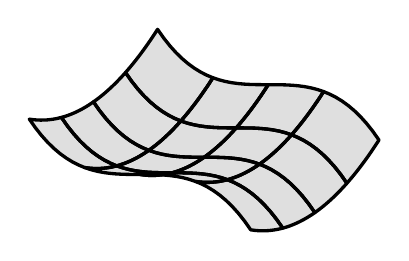
\begin{tikzpicture}[
    x=(215:2em/sqrt 2), y=(0:2em), z=(90:2em),
    declare function={f(\x,\y)=((\x-3)^2+(-\y+3)^3)/8+3;}, 
  very thick, line join=round]
%  \draw [-stealth, black!75] (0,0,0) -- (5,0,0) node [below left] {$x$};
%  \draw [-stealth, black!75] (0,0,0) -- (0,5,0) node [below right] {$y$};
%  \draw [-stealth, black!75] (0,0,0) -- (0,0,5) node [right] {$z$};

  \foreach \x in {1,...,4}
  \foreach \y in {1,...,4}{
    \draw [black, fill=black, fill opacity=0.125, 
    domain=0:1, samples=10, variable=\t] 
    plot (\x+\t, \y, {f(\x+\t,\y)}) -- 
    plot (\x+1, \y+\t, {f(\x+1,\y+\t)}) -- 
    plot (\x+1-\t, \y+1, {f(\x+1-\t,\y+1)}) --
    plot (\x, \y+1-\t, {f(\x,\y+1-\t)}) -- cycle;
  }
\end{tikzpicture}

  }
  \caption{\label{fig:dg:differenial_geometry}}
\end{figure}

\section{Coordinates}
Curved spacetime is a collection of events (or points) $p$ in a manifold $\mathcal{M}$. Semi-global patches of it may have their events labelled with coordinates $x^a = x^a(p)$, which are always ``upstairs'' indexed. Since we are in $1+3$ spacetime, typically, $a=0$ will denote a time-like coordinate, and $a=1,2,3$ space-like coordinates.

Technically, a coordinate is a scalar field defined on the manifold. A coordinate system is a set of scalar fields which provide a one-to-one mapping semi-global mapping from $\mathbb{R}^4$ to $\mathcal{M}$.

We will suppress indices on coordinates when the meaning is clear, for example in the case of a scalar field $\phi$ we write:
\begin{equation}
  \phi(x^a) = \phi(x)
  \label{eqn:dg:scalar_supress}
\end{equation}


%In general, the points $p\in \mathcal{M}$ will not form a vector space, and they cannot be added to one another in a meaningful way. Whilst there may be a physically meaningful addition and scaling of points in flat spacetimes, in the more general case there is not. For example, consider the manifold defined by the surface of the two-dimensional sphere $\mathcal{M}=S^2$. It is not possible to find an addition which is commutative and scalable

\section{Vectors}
This coordinate system defines a {\em contravariant\/} set of basis vectors at each point $\ve_a = \ve_a(p)$. Here the basis vector $\ve_a(p)$ is tangent to the coordinate curve:
\begin{equation}
  \gamma^a = \{x^b=\mathrm{const} : a\ne \nu\},
  \label{eqn:dg:coordinate_curve}
\end{equation}
at the point $p$.\footnote{Experienced readers will know that this notion is normally regarded as far from trivial.}
  Vectors at {\em at a given point\/} $p$ form a vector space which may be summed and scaled. Thus, a general vector $\vv$ may be written as a linear combination of basis vectors $\vv = v^a \ve_a$, where we use Einstein's summation convention that repeated upstairs and downstairs indices should be summed over. In addition, these vectors are equipped with a dot-product $\vv\cdot\vw$ which encapsulates the geometry of the vectors; namely spacetime angles and magnitudes. If a coordinate system is chosen, then:
\begin{equation}
  \vv\cdot\vw = (v^a\ve_a)\cdot(w^b\ve_b) = v^a (\ve_a\cdot\ve_b)w^b =  v^a g_{ab} w^b
  \label{eqn:dg:dot_product}
\end{equation}
where 
\begin{equation}
  g_{ab} = \ve_a\cdot\ve_b
  \label{eqn:dg:metric_def}
\end{equation}
is the {\em metric}, and is simply the dot product at a given point, expressed in a specific coordinate system.

Once a dot product is defined, it is convenient to define a set of {\em covariant\/} basis vectors $\{\ve^a\}$ via:
\begin{equation}
  \ve^a \cdot \ve_b = \delta^a_b 
  \qquad\Leftrightarrow\qquad
  \ve^a = g^{ab} \ve_b,
  \label{eqn:dg:covariant_basis}
\end{equation}
where $g^{ab}$ is the upstairs version of \eqref{eqn:dg:metric_def}, and by simple linear algebra is the matrix inverse of $g_{ab}$. Now that a dot product is defined, the covariant basis vector $\ve^a$ can be thought of as orthogonal to the coordinate surface $x^a=\mathrm{const}$. Materials scientists should recognise the covariant basis as simply the reciprocal basis. 

We can choose to write vectors in either the covariant or contravariant basis:
\begin{equation}
  \vv=v^b \ve_b = v_a \ve^a 
  \qquad\Rightarrow\qquad
  v_a = g_{ab} v^b.
  \label{eqn:dg:covariant_vector}
\end{equation}
The metric can therefore be used to ``raise'' or ``lower'' indices of vectors. The fact that the metric performs this operation should be intuitively obvious, since raised or lowered indexed vectors correspond to placing the vector in the covariant or contravariant coordinate system, whose definition \eqref{eqn:dg:covariant_basis} is defined via the dot-product.

\section{Tensors}
A Tensor $T$ is a multi-linear mapping of vectors onto a scalar at a given point:
\begin{align}
  \uT 
  &= 
  \uT(\va,\:\vb,\ldots,\:\vz)
  &
  \nonumber
  \\
  &= 
  \uT(a^\alpha\ve_\alpha,\:b^\beta\ve_\beta,\ldots,z^\zeta\ve_\zeta)  
  &\text{vectors in coordinate basis}
  \nonumber
  \\
  &= 
  a^\alpha b^\beta \ldots z^\zeta \: 
  \uT(\ve_\alpha,\:\ve_\beta,\:\ldots,\:\ve_\zeta)  
  &\text{apply multi-linearity}
  \nonumber
  \\
  T_{\alpha,\beta,\ldots,\zeta} 
  &=  
  T(\ve_\alpha,\:\ve_\beta,\:\ldots,\:\ve_\zeta)
  &\text{define a new set of numbers}
  \nonumber
  \\
  \Rightarrow\qquad
  \uT
  &= 
  a^\alpha b^\beta \ldots z^\zeta \: 
  T_{\alpha,\beta,\ldots,\zeta}
  &
  \nonumber
\end{align}
Upstairs components of a vector are defined similarly. It is interesting (although not surprising) that the metric is also a tensor, albeit a very special one which defines the geometry. The mapping is coordinate independent, but components are produced when a specific coordinate basis is chosen for each ``slot'' (each of which may be covariant or contravariant).

A mapping of a rank $m$ tensor onto a rank $n$ tensor may be produced from a rank $m+n$ tensor by simply leaving $n$ of the slots blank. In this sense, a vector can be considered as a rank $1$ tensor, its linear action defined by the dot product.

\section{Calculus}
So far, all we have discussed is a way of dealing with vectors whose bases are defined by an arbitrary coordinate system. The maths becomes interesting when we start to ask questions about how these vectors change from point to point on the manifold.

For scalar fields, the partial derivative is easy to define and calculate.

For a vector field:
\begin{equation}
 \vv(x) = v^a(x)\ve_a(x),
  \label{eqn:dg:vector_field}
\end{equation}
the problem is not so straightforward. First we now have two dependencies on position $x$, one in the field's components, and one in its basis vectors. Worse, we have no means of subtracting or adding vectors at different points in a manifold, so the traditional definition using ``small changes'' is useless. Nonetheless, if we attempt to find the partial derivative of this field:
\begin{equation}
  \partial_a\vv = \partial_a(v^b\ve_b) \equiv (\partial_a v^b) \ve_b + v^b \partial_a\ve_b
  \label{eqn:dg:partial_expand}
\end{equation}
we find that the only bit that we should be confused about is the final term involving the partial derivative of the basis vector. We have no means of computing this (yet), but it is certainly true that it will be a linear combination of the basis vectors:
\begin{equation}
  \partial_a\ve_b = \Gamma^c_{ba} \ve_c.
  \label{eqn:dg:gamma_def}
\end{equation}
The $\Gamma$ coefficients here are termed {\em Christoffel symbols}, and despite the notation are not the components of a tensor. We may also compute $\partial_a \ve^b$ by considering:
\begin{align}
  0 = \partial_a \delta^b_c &= \partial_a (\ve^b\cdot\ve_c)  
  \nonumber\\
  &= (\partial_a\ve^b)\cdot\ve_c + \ve^b\cdot(\partial_a\ve_c)
  \nonumber \\
  &= (\partial_a\ve^b)\cdot\ve_c + \ve^b\cdot\Gamma^d_{ca} \ve_d 
  \nonumber \\
  &= (\partial_a\ve^b)\cdot\ve_c + \Gamma^d_{ca} \delta^b_d
  \nonumber \\
  &= (\partial_a\ve^b)\cdot\ve_c + \Gamma^b_{ca} 
  \nonumber \\
  &= (\partial_a\ve^b)\cdot\ve_c + \Gamma^b_{ca} 
  \nonumber \\
  \Rightarrow \partial_a\ve^b
  &=  - \Gamma^b_{ca} \ve^c
  \label{eqn:dg:chris_deriv}
\end{align}
With this, we may define a new {\em covariant derivative\/} for vector fields such that:
\begin{align}
  \partial_a\vv &= (\nabla_a v^b) \ve_b = (\nabla_a v_b) \ve^b,
  \\
   \nabla_a v^b &= \partial_a v^b + \Gamma^b_{ca}v^c,
   \\
   \nabla_a v_b &= \partial_a v_b - \Gamma^c_{ba}v_c.
\end{align}
Tensors may be defined similarly so that
\begin{align}
  \partial_a \uT &= (\nabla_a T^{bc}),
  \\
  \nabla_a T^{bc} &= \partial_a T^{bc} + \Gamma^b_{da}T^{dc} + \Gamma^c_{da}T^{bd},
\end{align}
with similar formulae for downstairs components.

All that remains is to find out what the Christoffel symbols actually are. Demanding metric compatibility and torsionlessness yields:
\begin{equation}
  \Gamma^a_{bc} = \frac{1}{2}g^{ad}
  \left( 
  \partial_b g_{dc} 
  +\partial_c g_{bd} 
  -\partial_d g_{bc} 
  \right)
  \label{eqn:dg:christoffel}
\end{equation}

We define the curvature tensor as
\begin{align}
  R^d_{abc} v_d &= \left( \nabla_{bc} - \nabla_{cb} \right) v_a
  \label{eqn:dg:riemann_def}\\
  R^d_{abc} &= \partial_b \Gamma^d_{ac} - \partial_c \Gamma^d_{ab} + \Gamma^e_{ac}\Gamma^d_{ab} - \Gamma^e_{ab}\Gamma^d_{ec}
\end{align}

The Ricci tensor is defined as:
\begin{equation}
  R_{ab} = R^d_{dab}
  \label{eqn:dg:ricci_tensor}
\end{equation}

The Ricci scalar is defined as:
\begin{equation}
  R = R^a_a
  \label{eqn:dg:ricci_scalar}
\end{equation}







